\section{Results}
    All simulations and consequent plots and figures up until Figure \ref{jupitermass1000} has been done with the Sun fixed to the origin, unable to move as a result of the force acting on it from other bodies in the system.
\subsection{Numerical error and run times}
	\begin{table}[h!]
		\centering
		\caption{Tabular overview of sequential run times for increasing number of integration points $N$ for each solver when solving the motion equation for Earth in the Earth - Sun system.}
		\label{runtime}
		\begin{tabular}{l|l|l|l}
			$N$ & Euler-Forward [s] & Euler-Cromer [s] & Velocity Verlet [s]\\
			\hline
			10$^1$ &3.04$\cdot10^{-4}$ & 1.57$\cdot10^{-4}$ &2.68$\cdot10^{-4}$\\
			10$^2$ &9.29$\cdot10^{-4}$ & 6.80$\cdot10^{-4}$ &7.23$\cdot10^{-4}$ \\
			10$^3$ &6.70$\cdot10^{-3}$ & 6.89$\cdot10^{-3}$ &8.50$\cdot10^{-3}$\\
			10$^4$ &5.96$\cdot10^{-2}$ & 6.18$\cdot10^{-2}$ &6.65$\cdot10^{-2}$ \\
			10$^5$ &5.98$\cdot10^{-1}$ &5.64$\cdot10^{-1}$ &6.54$\cdot10^{-1}$ \\
			10$^6$ & 5.98$\cdot10^0$& 5.58 $\cdot10^0$&6.79$\cdot10^0$ \\
			10$^7$ &6.60$\cdot10^1$ &6.59$\cdot10^1$ &6.75$\cdot10^1$
			
		\end{tabular}
	\end{table}
	\begin{figure}[h!]
		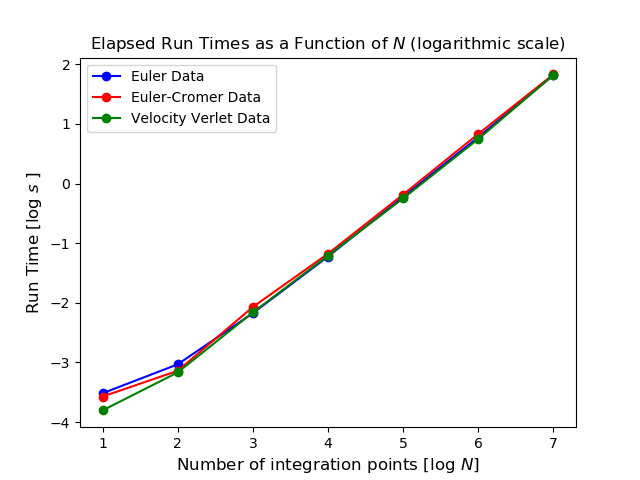
\includegraphics[width = \linewidth]{Figure/runtimes_proj3.png}
		\caption{A plot showing the relationship between the number of integration points $N$ and the elapsed run times for each of the three solvers as to illustrate the different solvers' efficiency.}
		\label{runtimes_plot}
	\end{figure}
	Figure \ref{runtimes_plot} and Table \ref{runtime} both illustrate the numerical efficiency of each of the different solvers we have studied in this project. The main observation here is that the elapsed run times follow a linear relationship with the number of integration points which is what we would expect from the number of FLOPs each solver carries with them. Second to that we see that there are very small differences in the data, reflecting the relatively small differences in FLOPs for each algorithm. 
	\newpage
	\begin{table}[H]
		\centering
		\caption{Tabular overview of the maximum numerical error for a given number of integration points $N$ for each solver when solving the motion equation for Earth in the Earth - Sun system.}
		\label{error}
		\begin{tabular}{l|l|l|l}
			$N$ & Euler-Forward & Euler-Cromer & Velocity Verlet\\
			\hline
			10$^1$ &4.19$\cdot10^0$ &5.31$\cdot10^{-1}$ & 1.87$\cdot10^{-1}$\\
			10$^2$ &7.17$\cdot10^{-1}$ &3.34$\cdot10^{-2}$ &1.97$\cdot10^{-3}$ \\
			10$^3$ &7.69$\cdot10^{-2}$ &3.14$\cdot10^{-3}$ &1.97$\cdot10^{-5}$ \\
			10$^4$ &7.87$\cdot10^{-3}$ &3.15$\cdot10^{-4}$ &1.97$\cdot10^{-7}$ \\
			10$^5$ & 7.89$\cdot10^{-4}$&3.29$\cdot10^{-5}$ &1.97$\cdot10^{-9}$ \\
			10$^6$ &7.89$\cdot10^{-5}$ &1.74$\cdot10^{-5}$ &1.97$\cdot10^{-11}$ \\
			10$^7$ &1.40$\cdot10^{-5}$ &2.02$\cdot10^{-5}$ & 7.65$\cdot10^{-14}$ 
		\end{tabular}
	\end{table}
	\begin{figure}[H]
		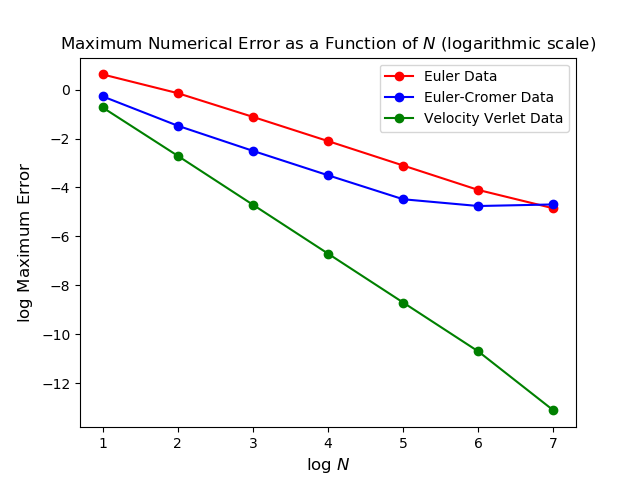
\includegraphics[width=\linewidth]{Figure/maxerrorplot_proj3.png}
		\caption{A plot showing the relationship between the number of integration points $N$ and the maximum numerical error for each of the three solvers as to illustrate the different solvers' precision. }
		\label{maxerror_plot}
	\end{figure}
	
	\begin{table}[H]
		\centering
		\caption{Tabular overview of the maximum numerical error for a given number of years for each solver when solving the motion equation for Earth in the Earth - Sun system with a constant $N = 10^{5}$.}
		\label{error_constN}
		\begin{tabular}{l|l|l|l}
			Years & Euler-Forward & Euler-Cromer & Velocity Verlet\\
			\hline
			10$^0$ &7.89$\cdot10^{-4}$&3.29$\cdot10^{-5}$ &1.97$\cdot10^{-9}$\\
			10$^1$ &7.33$\cdot10^{-2}$ &3.15$\cdot10^{-4}$ &1.97$\cdot10^{-7}$ \\
			10$^2$ &1.94$\cdot10^{0}$ &3.14$\cdot10^{-3}$ &1.97$\cdot10^{-5}$ \\
			10$^3$ &2.58$\cdot10^{1}$ &4.2$\cdot10^{-2}$ &1.97$\cdot10^{-3}$ \\
			10$^4$ & 4.16$\cdot10^{4}$&3.25$\cdot10^{3}$ &1.88$\cdot10^{-1}$ \\
			10$^5$ &3.99$\cdot10^{6}$ &3.99$\cdot10^{6}$ &2.06$\cdot10^{6}$
		\end{tabular}
	\end{table}
	\begin{figure}[H]
		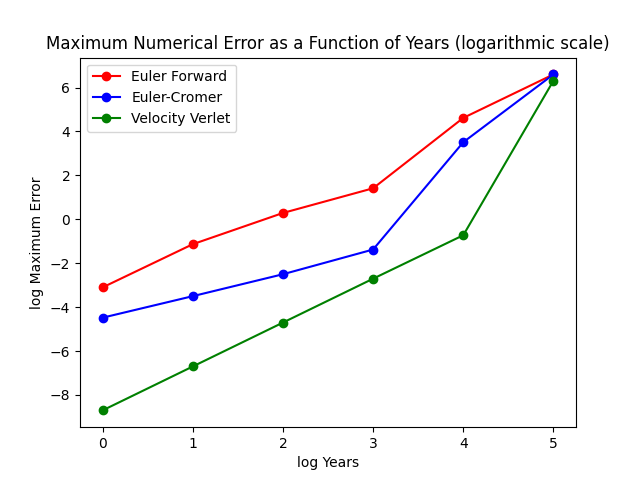
\includegraphics[width = \linewidth]{Figure/maxerrorplotconstN.png}
		\caption{A plot showing the relationship between the number of Years and the maximum numerical error for each of the three solvers}
		\label{maxerrorconstN_plot}
	\end{figure}

	Figure \ref{maxerror_plot} and Table \ref{error} illustrate the numerical precision of each of the three solvers. The data in Table \ref{error} is in itself implicative of the Verlet - algorithms superiority in this setting. As was mentioned in the sections for each of the different algorithms, the two Euler methods both commit a first-order global truncation error $\mathcal{O}(h)$, whilst the Velocity Verlet method commits a second-order global truncation error $\mathcal{O}(h^2)$ - these are all reflected in Figure \ref{maxerror_plot}. It is easy to extract by visual observation that the error in the two Euler methods decreases linearly with a gradient close to one, and that the error in the Verlet method decreases twice as fast with a gradient close to two. The computed gradients are -0.94, -1.04 and -2.04 for the Euler-Forward, Euler-Cromer and Velocity Verlet algorithms respectively. Here we have omitted the anomalous data for the error in the Euler-Cromer method for $N > 10^5$ when making linear fits.\\ 

	\newpage
	\begin{figure}[h!]
		\centering
		\begin{subfigure}{0.49\linewidth}
			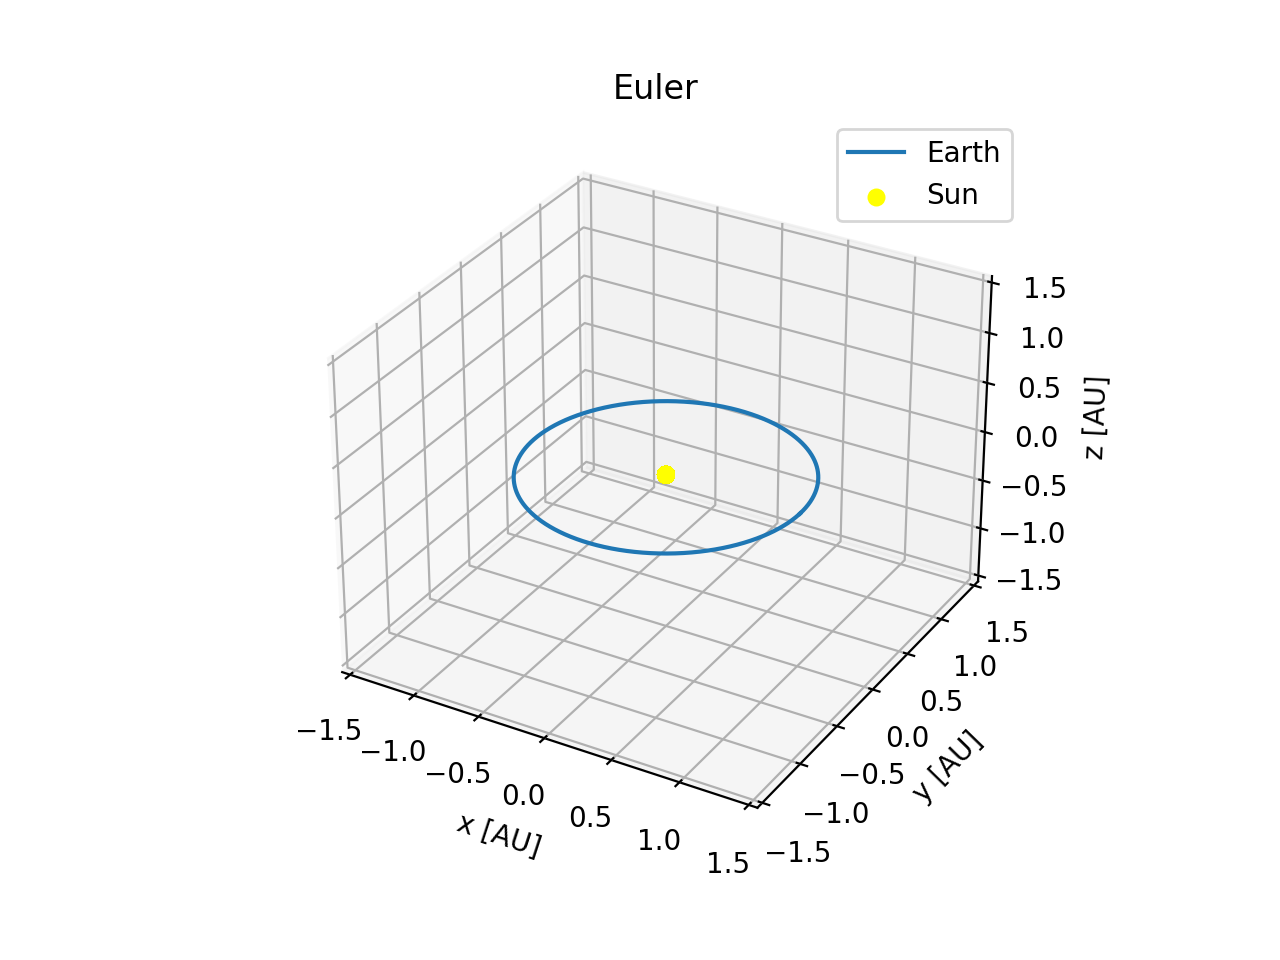
\includegraphics[width=1.15\linewidth]{Figure/euler_forward_oneyear.png}
		\end{subfigure}
		\begin{subfigure}{0.49\linewidth}
			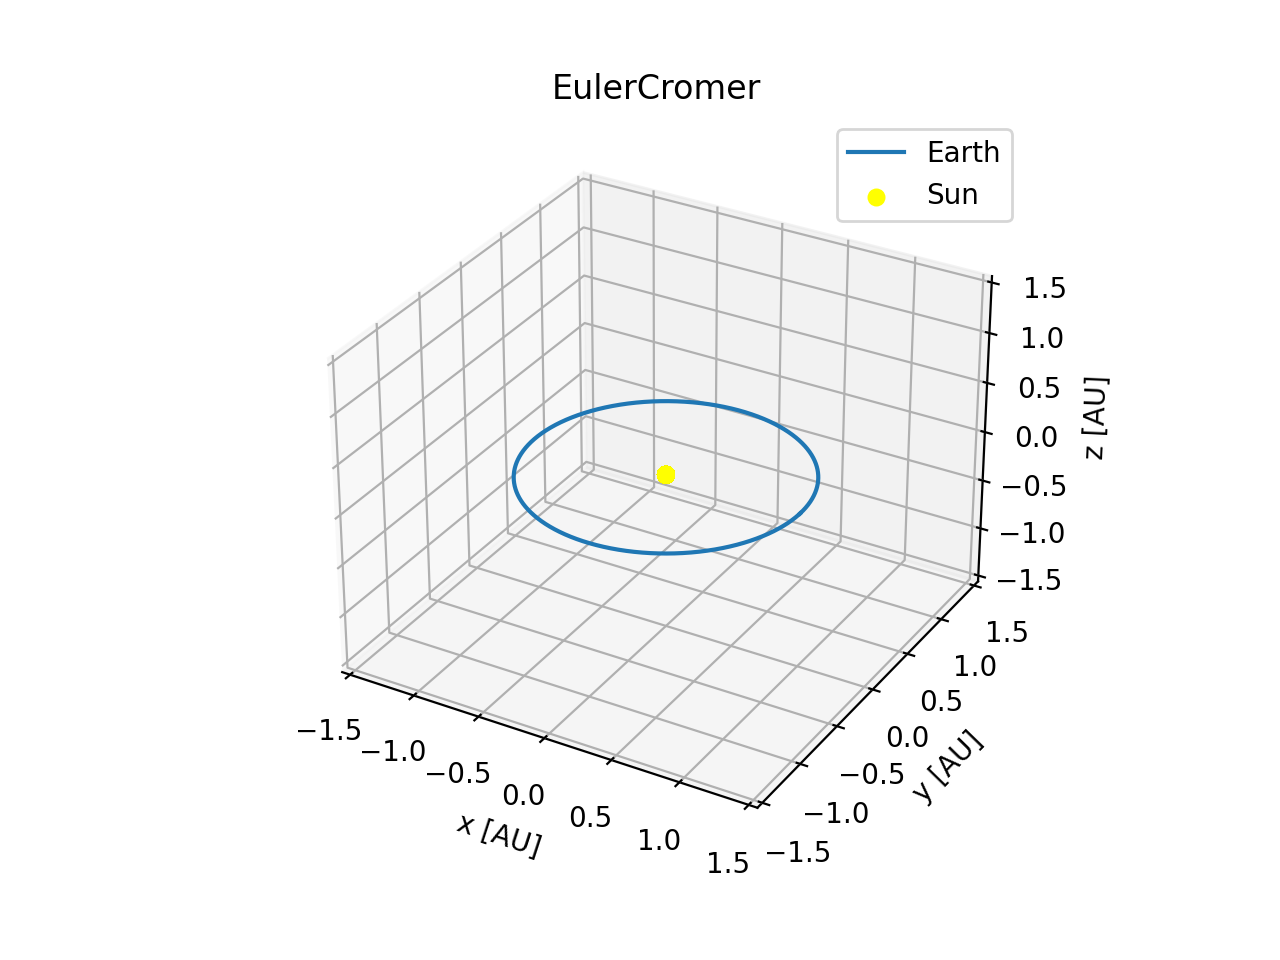
\includegraphics[width=1.2\linewidth]{Figure/euler_cromer_oneyear.png}
		\end{subfigure}
	\caption{3D plots of Earth's annual orbit around the Sun as calculated by the Euler - Forward (left) and Euler - Cromer (right) algorithms for $N = 10^6,\ h = 10^{-6}$. }
	\label{eulers3doneyear}
	\end{figure}
	\begin{figure}[h!]
		\centering
		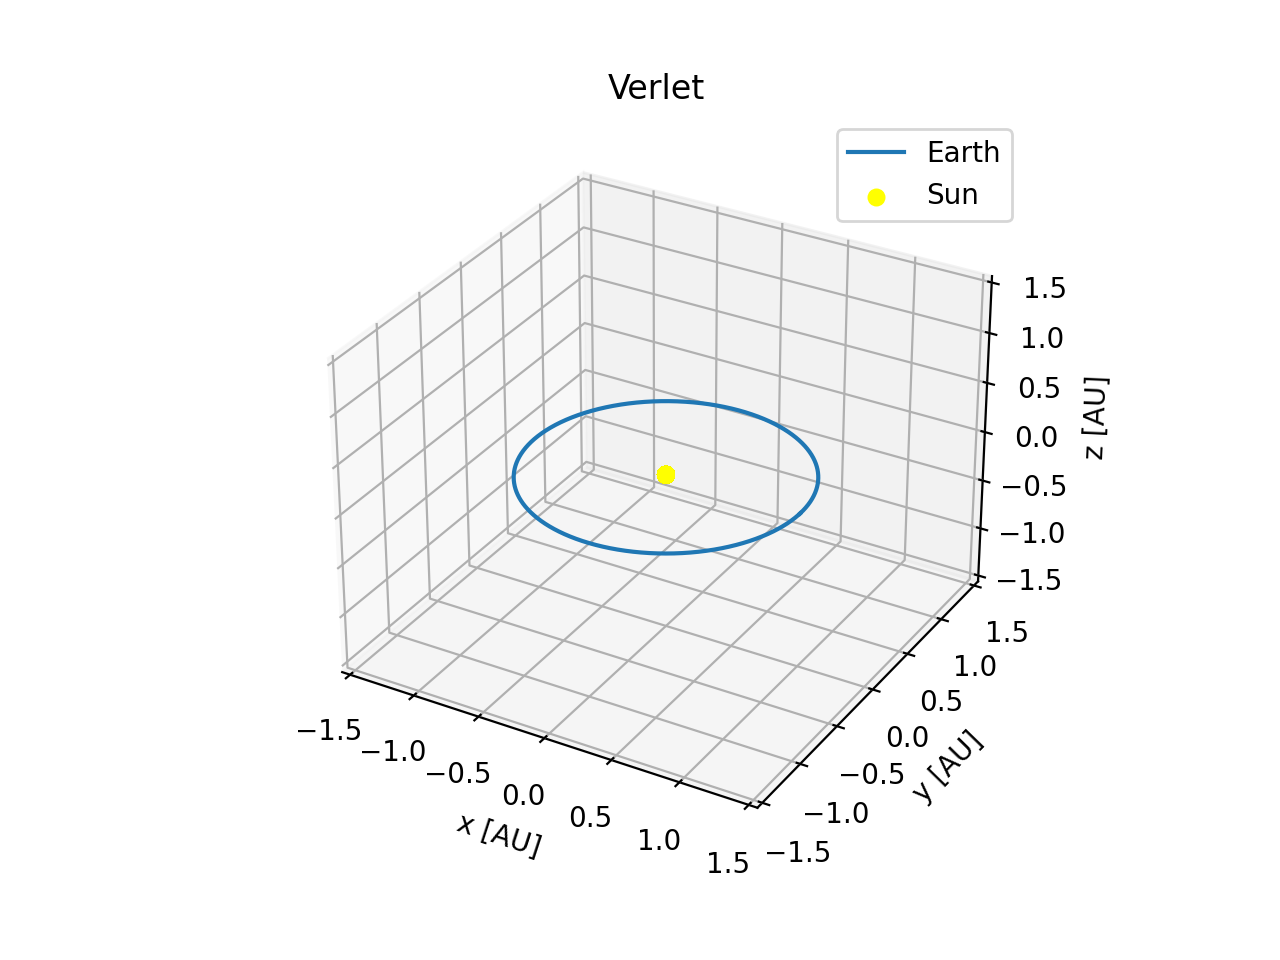
\includegraphics[width=0.6\linewidth]{Figure/verlet_oneyear.png}
		\caption{3D plot of Earth's annual orbit around the Sun as calculated by the Velocity Verlet algorithm for $N = 10^6,\ h = 10^{-6}$.}
		\label{verlet3doneyear}
	\end{figure}
	\newpage

	\begin{figure}[h!]
		\centering
		\begin{subfigure}{0.48\linewidth}
			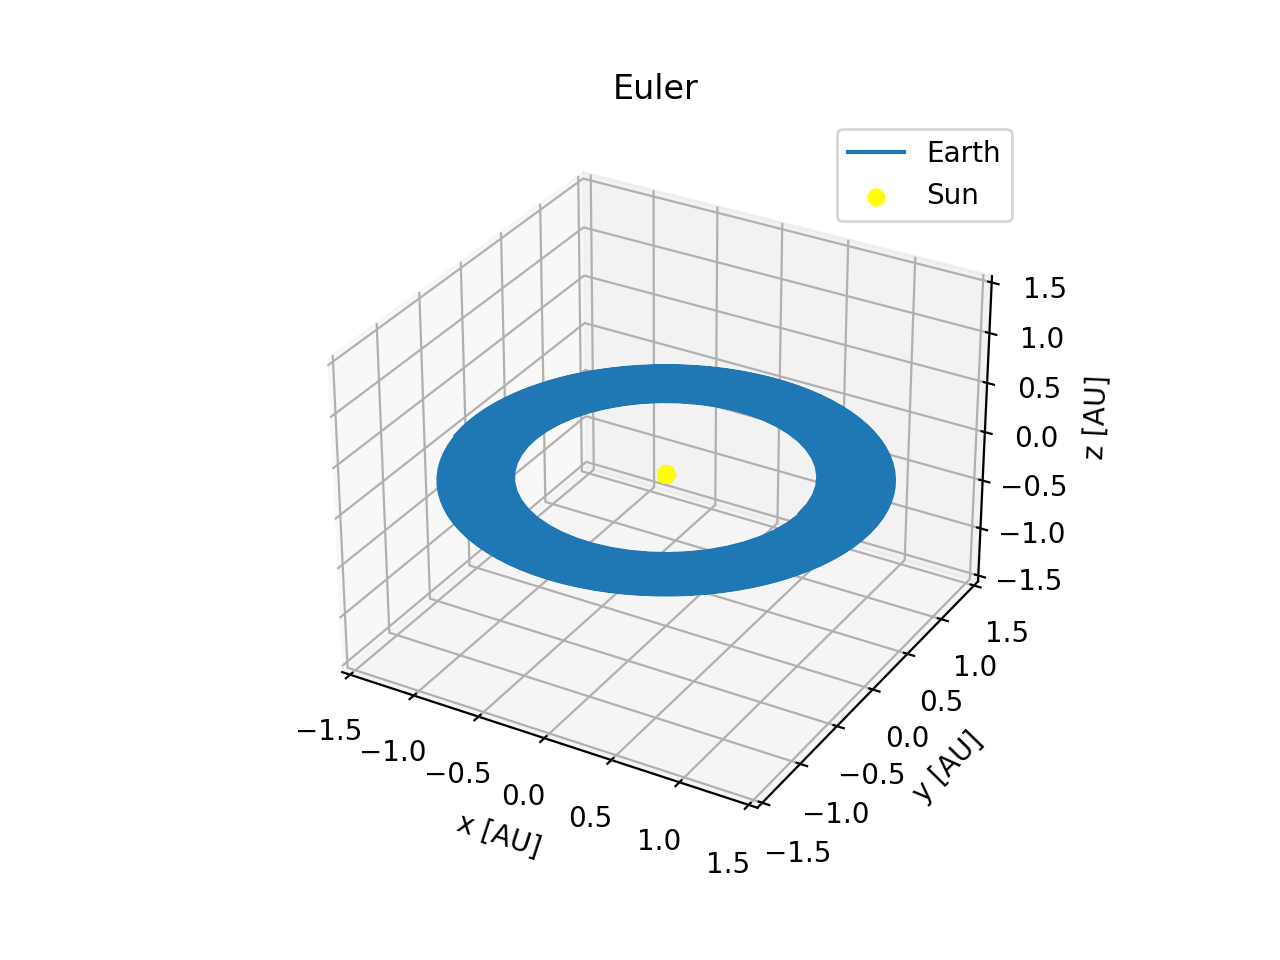
\includegraphics[width=1.2\linewidth]{Figure/euler_forward_100years.png}
		\end{subfigure}
		\begin{subfigure}{0.48\linewidth}
			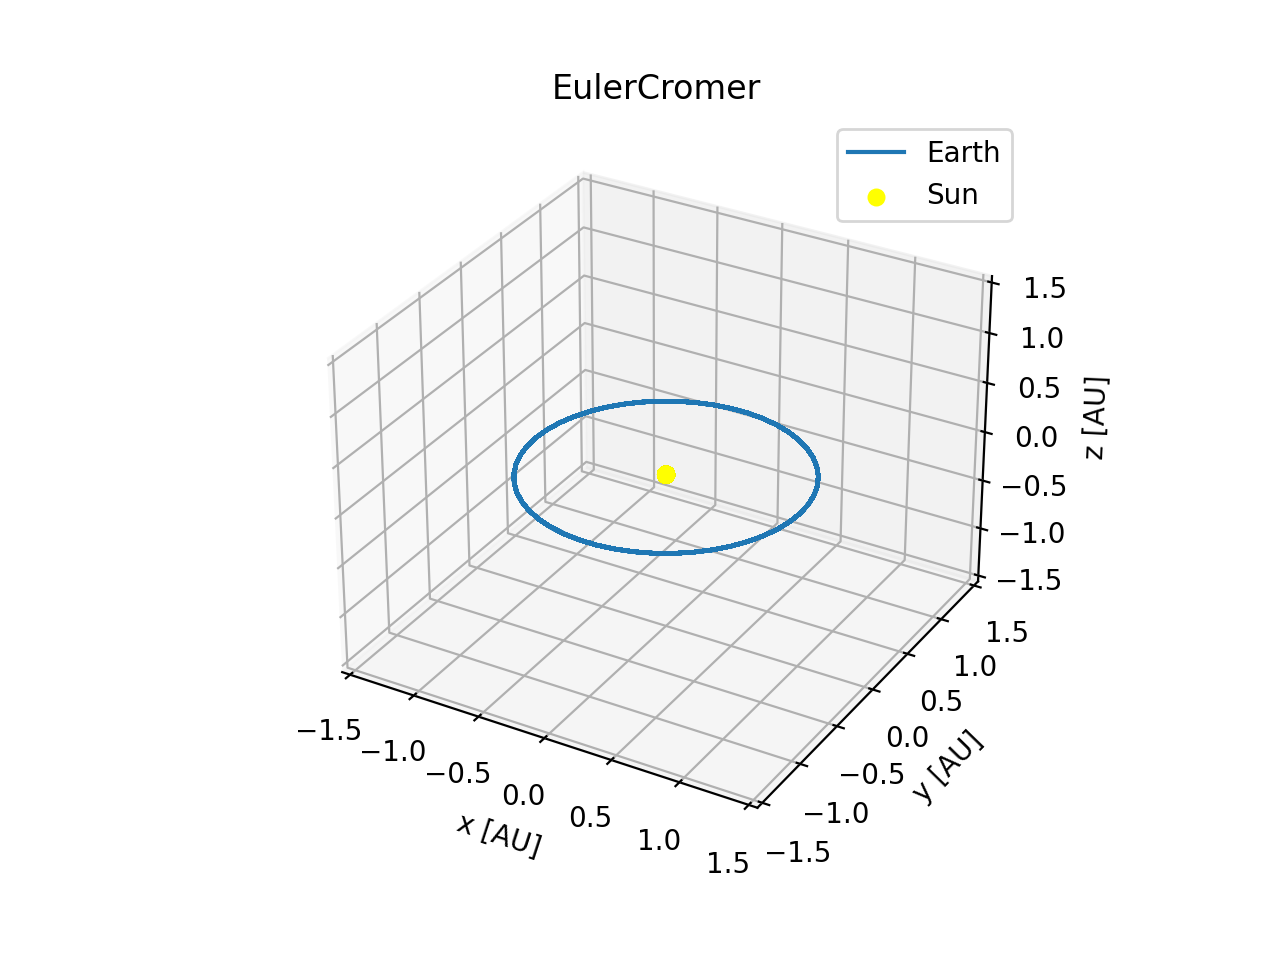
\includegraphics[width=1.15\linewidth]{Figure/eulercromer_100years.png}
		\end{subfigure}
		\caption{3D plots of Earth's centennial orbit around the Sun as calculated by the Euler - Forward (left) and Euler - Cromer (right) algorithms  for $N = 10^6,\ h = 10^{-4}$. }
		\label{eulers3100year}
	\end{figure}
	\begin{figure}[h!]
		\centering
		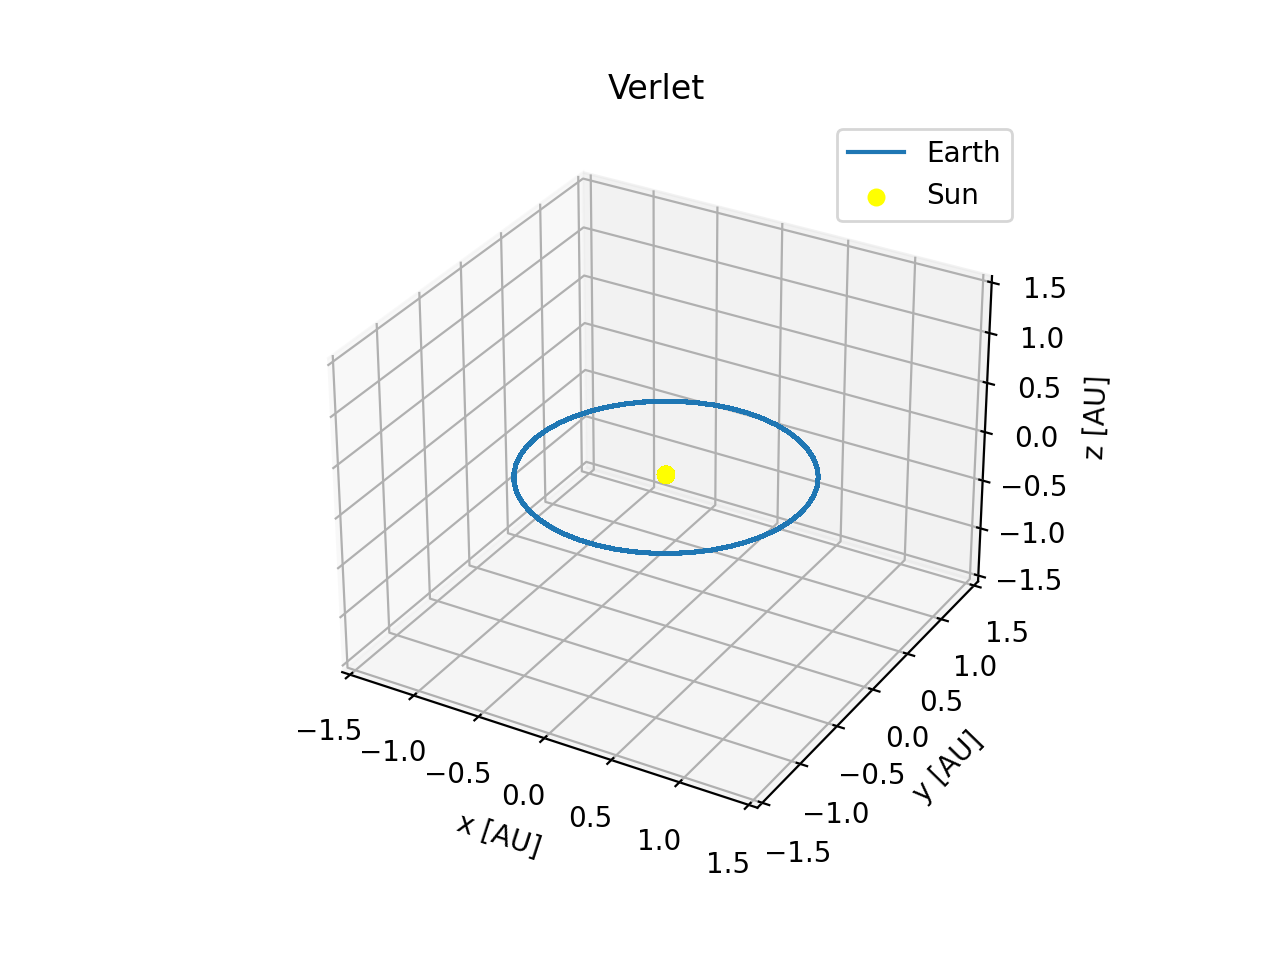
\includegraphics[width=0.6\linewidth]{Figure/verlet_100years.png}
		\caption{3D plot of Earth's centennial orbit around the Sun as calculated by the Velocity Verlet algorithm for $N = 10^6,\ h = 10^{-4}$.}
		\label{verlet3d100year}
	\end{figure}
	\newpage
	
	Figures \ref{eulers3doneyear} and \ref{verlet3doneyear} are simulations of Earth's annual motion around the Sun for a high temporal resolution $h = 10^{-6}$. In these plots, we should observe that the numerical precision is visually indistinguishable for the three solvers, and we would have to consult Tables \ref{error} and \ref{error_constN} to conclude that the Velocity Verlet algorithm indeed produces the most precise result. Now, Figures \ref{eulers3100year} and \ref{verlet3d100year} are simulations of Earth's centennial motion around the Sun, with a lower temporal resolution $h = 10^{-4}$. We immediately see that the Euler-Forward algorithm is non-symplectic as stated in Section 4.2. The orbital "width" indicates a motion in which the Earth strays from its (initialized) circular orbit of radius 1. The symplectic (energy conserving) Euler-Cromer and Velocity Verlet algorithms are still stable for this temporal resolution, and we see from Tables \ref{error} and \ref{error_constN}, as well as Figures \ref{maxerror_plot} and \ref{maxerrorconstN_plot} that a simulation of Earth's millennial motion in the Earth-Sun system would result in noticeably imprecise system, especially when devising the Euler-Cromer algorithm.\\ 
	
	\begin{figure}[H]
		\centering
		\begin{subfigure}{0.48\linewidth}
			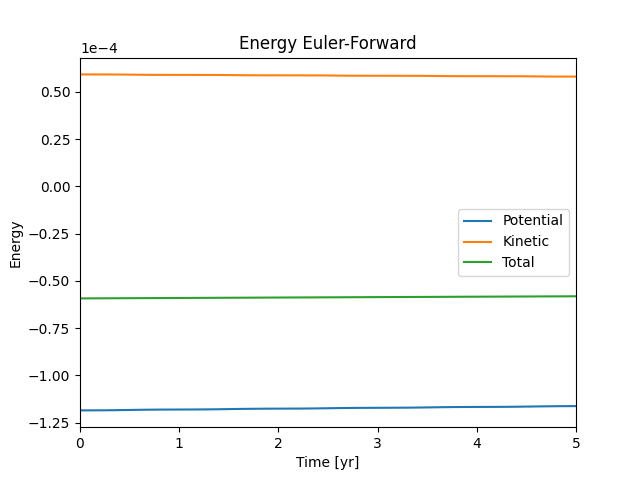
\includegraphics[width=1.1\linewidth]{Figure/EnergyEuler.png}
		\end{subfigure}
		\begin{subfigure}{0.48\linewidth}
			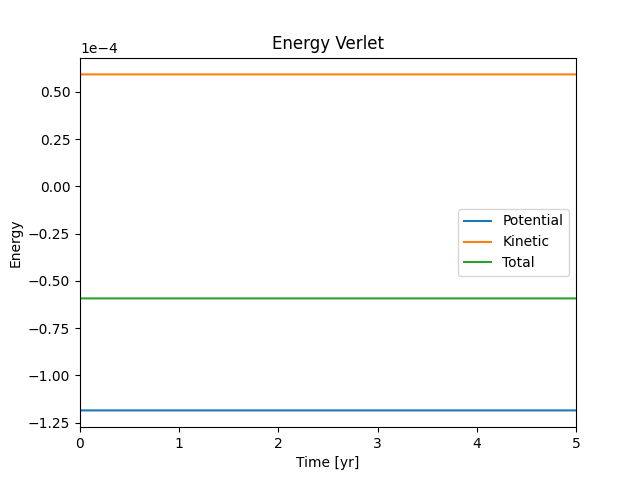
\includegraphics[width=1.1\linewidth]{Figure/EnergyVerlet.png}
		\end{subfigure}
		\caption{Plots of kinetic, potential and total energy for the Earth-Sun system for Euler-Forward (left) and Velocity Verlet (right) with $h = 5\cdot10^{-5}$.}
		\label{energy2body}
	\end{figure}

    Figure \ref{energy2body} exhibit the non-symplecticity of the Euler-Forward scheme, as can be seen, just by putting some good will to use, by the increase in total energy. For the Velocity Verlet algorithm, the total energy is conserved. \\ \\
    
    \begin{table}[H]
		\centering
		\caption{Tabular overview of the time step needed to have conservation of angular momentum with a tolerance of $10^{-10}$ for the Earth-Sun system.}
		\label{conservationtable}
		\begin{tabular}{|l|l|}
		    \hline
			Years & h\\
			\hline
			1 & 2.3$\cdot 10^{-3}$\\
			10 & 2.3$\cdot 10^{-3}$\\
			100 & 2.1$\cdot 10^{-3}$\\
			1000 & 1.1$\cdot 10^{-3}$\\
			\hline
		\end{tabular}
	\end{table}
	
   Table \ref{conservationtable} shows roughly what step length is needed to achieve conservation of angular momentum for the Earth-Sun system. \\
   
   The program has been written such that a value $\beta$ can be passed. This value corresponds to the exponent of $r$ in the gravitational force term. Values of $\beta \in [2,3]$ have been tested, in order to find out whether there can be forces other than the inverse-square force sustaining a stable Earth-Sun system. 

   \begin{figure}[H]
		\centering
		\begin{subfigure}{0.48\linewidth}
			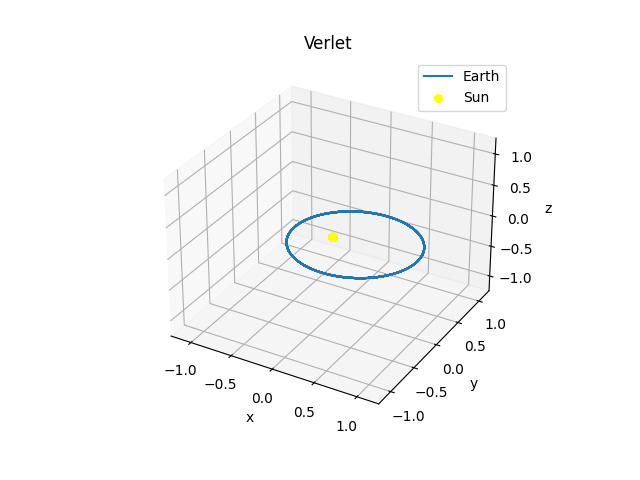
\includegraphics[width=1.2\linewidth]{Figure/Verlet_elliptical_B200.png}
			\caption{$\beta=2$}
		\end{subfigure}
		\begin{subfigure}{0.48\linewidth}
			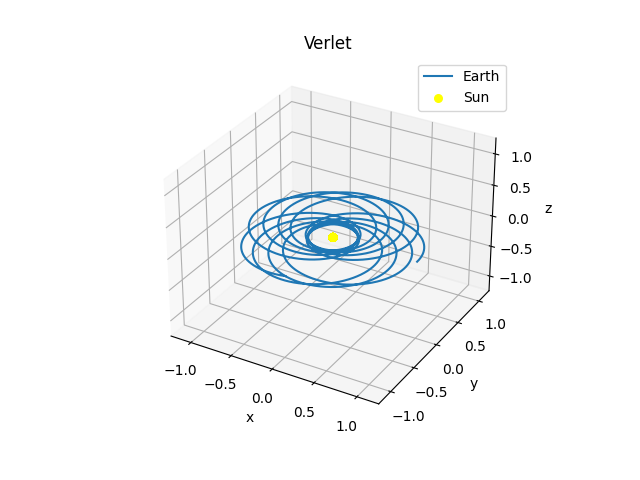
\includegraphics[width=1.15\linewidth]{Figure/Verlet_elliptical_B250.png}
			\caption{$\beta=2.5$}
		\end{subfigure}
		\begin{subfigure}{0.48\linewidth}
			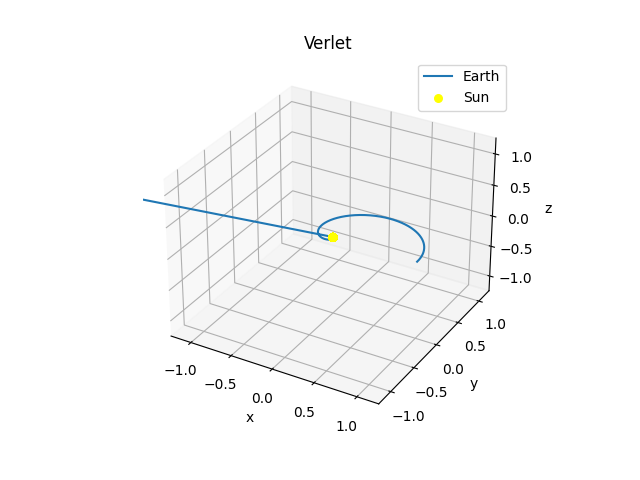
\includegraphics[width=1.15\linewidth]{Figure/Verlet_elliptical_B300.png}
			\caption{$\beta = 3$}
		\end{subfigure}
		\caption{Plots of the Earth-Sun system with a gravitational force $F \propto 1/r^{\beta}$, where $\beta\in[2,3]$. Earth's initial position is (0, 1 AU, 0) and velocity (5 AU/yr, 0, 0)}
		\label{betaelliptical}
	\end{figure}
	
	In Figure \ref{betaelliptical}, Earth is initiated with an elliptical orbit. For $\beta = 2.5$, the orbit looks chaotic and far from the observed orbit. For $\beta = 3$, Earth has a rapidly declining orbit, and since our program has no functionality to detect planets colliding, Earth moved past the Sun's center, and experiences a huge force which throws it out of the Solar system in the other direction. 
	
	\begin{figure}[H]
	    \centering
	    \begin{subfigure}{0.52\linewidth}
	        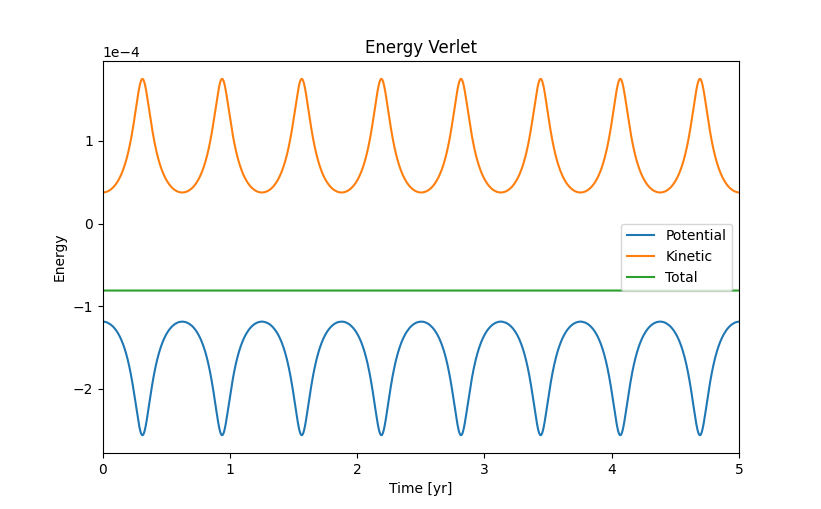
\includegraphics[width=1\linewidth]{Figure/VerletEnergy_elliptical_B200.png}
	        \caption{$\beta = 2$}
	   \end{subfigure}
	   \begin{subfigure}{0.45\linewidth}
	        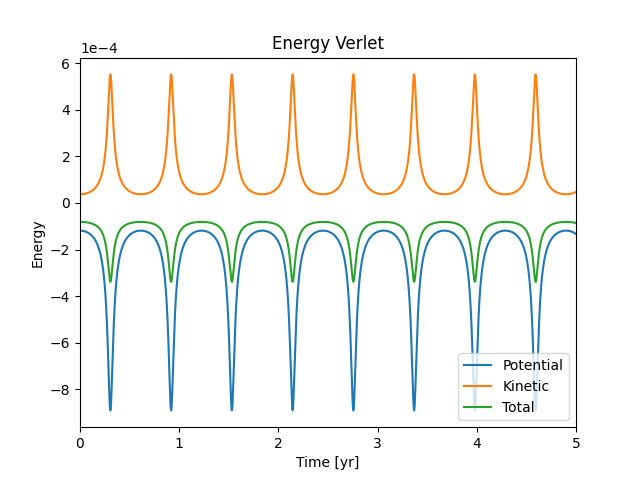
\includegraphics[width=1\linewidth]{Figure/VerletEnergy_elliptical_B250.png}
	        \caption{$\beta = 2.5$}
	   \end{subfigure}
	   \caption{Energies of elliptical orbit with varying $\beta$}
	   \label{EllipticalEnergy}
    \end{figure}
    
	
	An inspection of the total energies (Figure \ref{EllipticalEnergy} for the systems in Figure \ref{betaelliptical} reveals that with $\beta = 2.5$, the energy for the system is not conserved. It is however conserved with $\beta = 2$, as expected. We consider now a varying $\beta$ with an Earth initiated with a circular orbit.
	  
   \begin{figure}[H]
		\centering
		\begin{subfigure}{0.48\linewidth}
			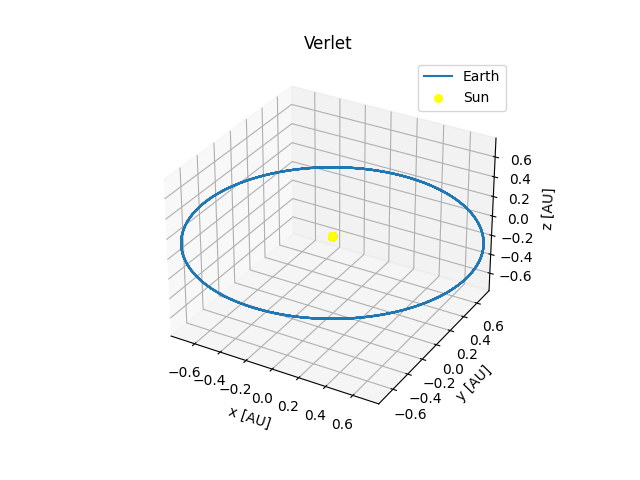
\includegraphics[width=1.2\linewidth]{Figure/Position_NASA_B201.png}
		\end{subfigure}
		\begin{subfigure}{0.48\linewidth}
			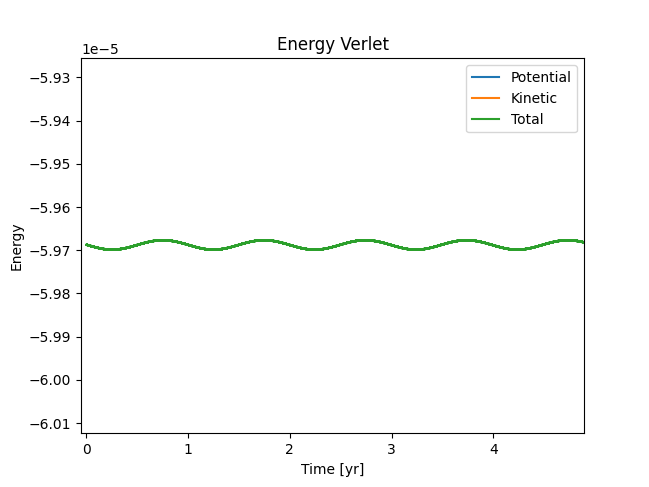
\includegraphics[width=1.15\linewidth]{Figure/Energy_NASA_B201.png}
		\end{subfigure}
		\caption{Plots of position (left) and energy (right) for Earth-Sun system with NASA data for initial position and velocity and $\beta = 2.01$}
		\label{B201_NASA}
	\end{figure}
	
	The position plot in Figure \ref{B201_NASA} does not raise cause for concern upon inspection. The energy plot tells a different story, as the total energy for the system can be seen to fluctuate in an oscillating fashion; the energy for the system is not conserved. We see no reason to include plots for higher values of $\beta$, as this energy fluctuation only increase in magnitude for increasing $\beta$. The program output also shows that angular momentum is not conserved for $\beta > 2$, and this is true for however small step size is chosen.
   
   \subsection{Escape Velocity}
   \begin{figure}[H]
		\centering
		\begin{subfigure}{0.48\linewidth}
			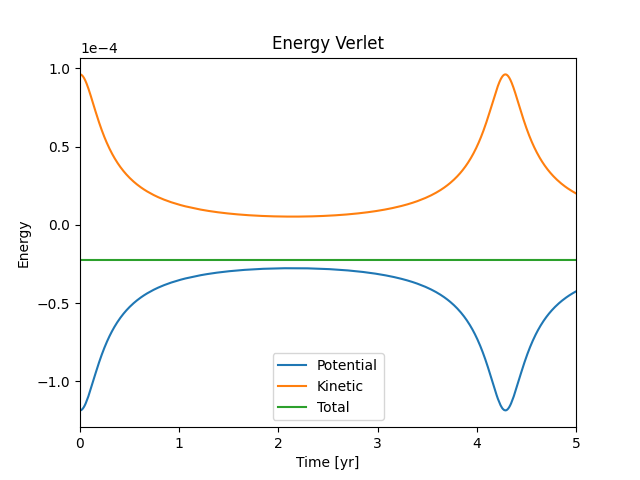
\includegraphics[width=1.2\linewidth]{Figure/EscVel_E_8.png}
			\caption{Energy with $V_0$ = 8 AU/yr}
		\end{subfigure}
		\begin{subfigure}{0.48\linewidth}
			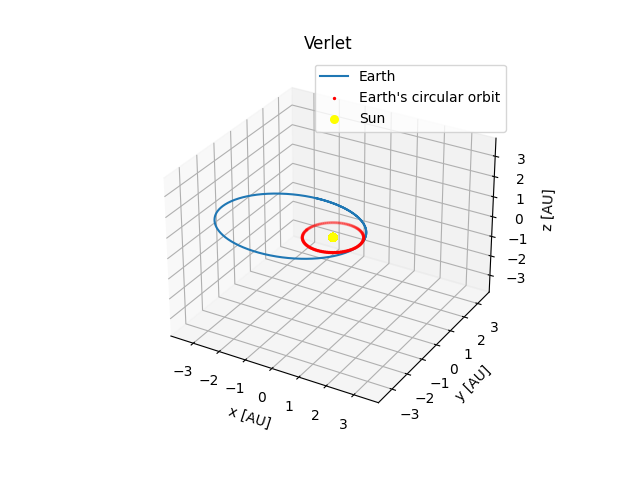
\includegraphics[width=1.15\linewidth]{Figure/EscVel_P_8.png}
			\caption{Position with $V_0$ = 8 AU/yr}
		\end{subfigure}
		\begin{subfigure}{0.48\linewidth}
			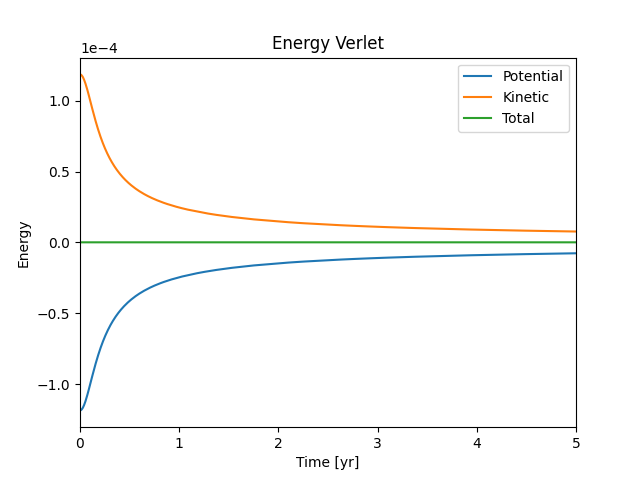
\includegraphics[width=1.15\linewidth]{Figure/EscVel_E_889.png}
			\caption{Energy with $V_0$ = 8.89 AU/yr}
		\end{subfigure}
		\begin{subfigure}{0.48\linewidth}
			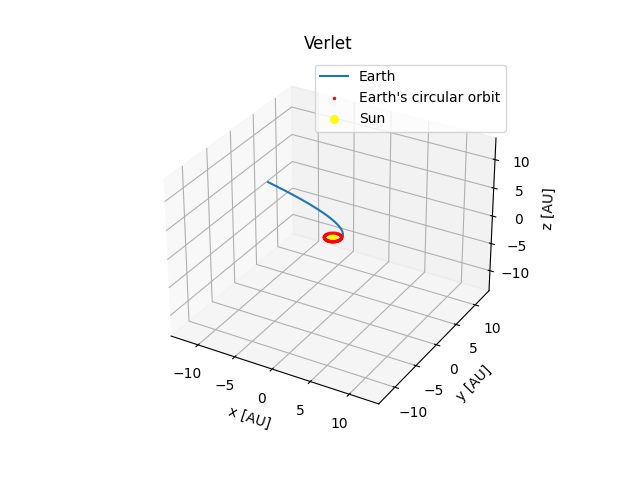
\includegraphics[width=1.15\linewidth]{Figure/EscVel_P_889.png}
			\caption{Position with $V_0$ = 8.89 AU/yr}
		\end{subfigure}
		\caption{Plots of the position and energy for different initial velocities}
		\label{EscVel_trial}
	\end{figure}
	
	Figure \ref{EscVel_trial} shows two runs with different initial velocities for Earth. In the top two plots, Earth has a initial velocity in y-direction of $8$ AU/yr. This produces an orbit with a semi major axis of more than 3 AU, but the Earth is still in orbit. In the bottom two plots, the initial velocity in y-direction is set to $8.89$ AU/yr. This is below the analytical value found in the Theory-section, and as can be seen from the energy plot, the total energy is above 0. This means that Earth is able to overcome the Sun's gravitational pull and escape the Solar system.
	
	\subsection{Three-Body System}

	\begin{figure}[h!]
		\centering
		\begin{subfigure}{0.48\linewidth}
			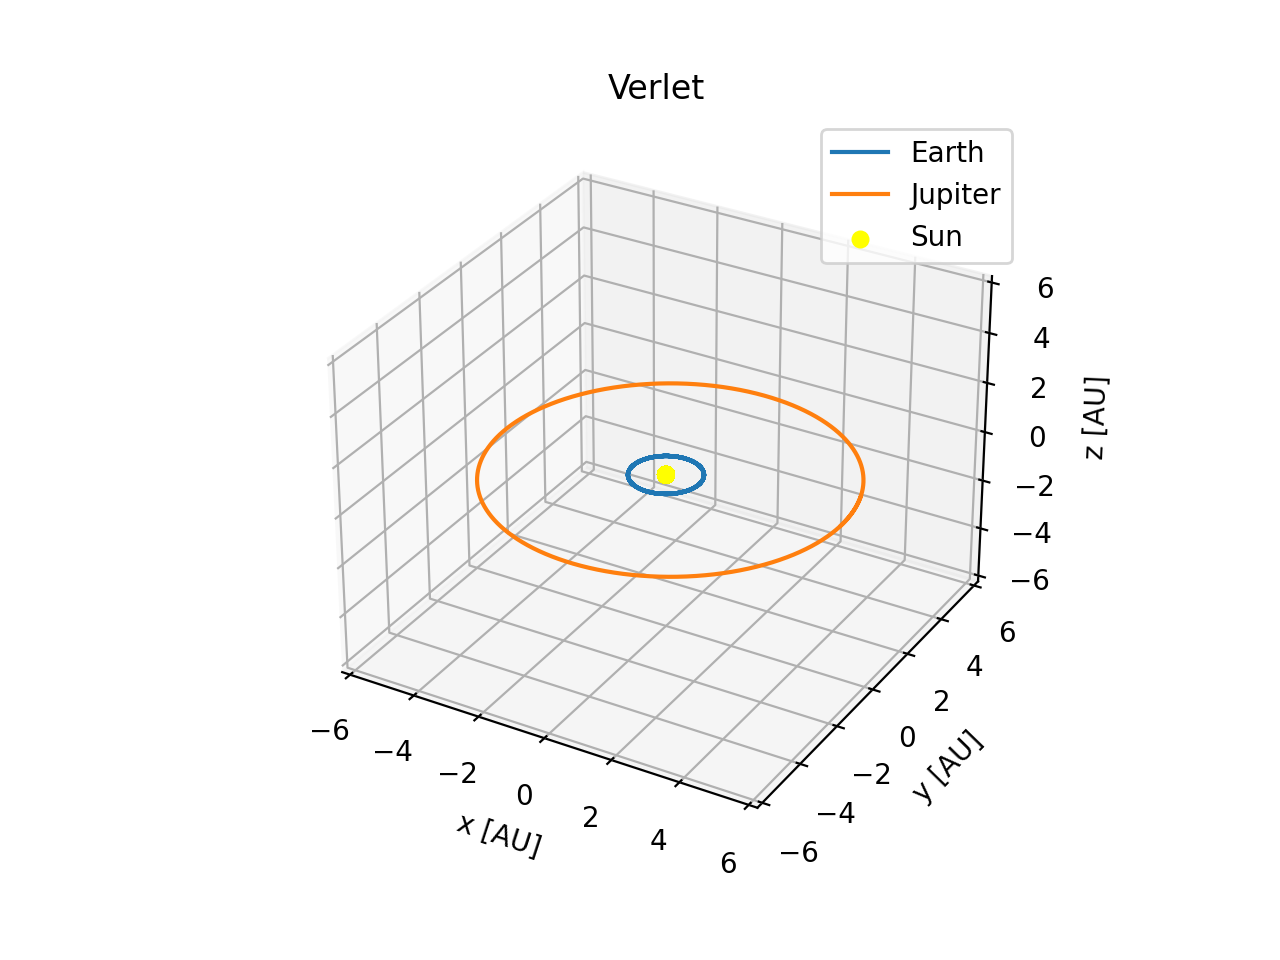
\includegraphics[width=1.2\linewidth]{Figure/threebodynormalmass.png}
		\end{subfigure}
		\begin{subfigure}{0.48\linewidth}
			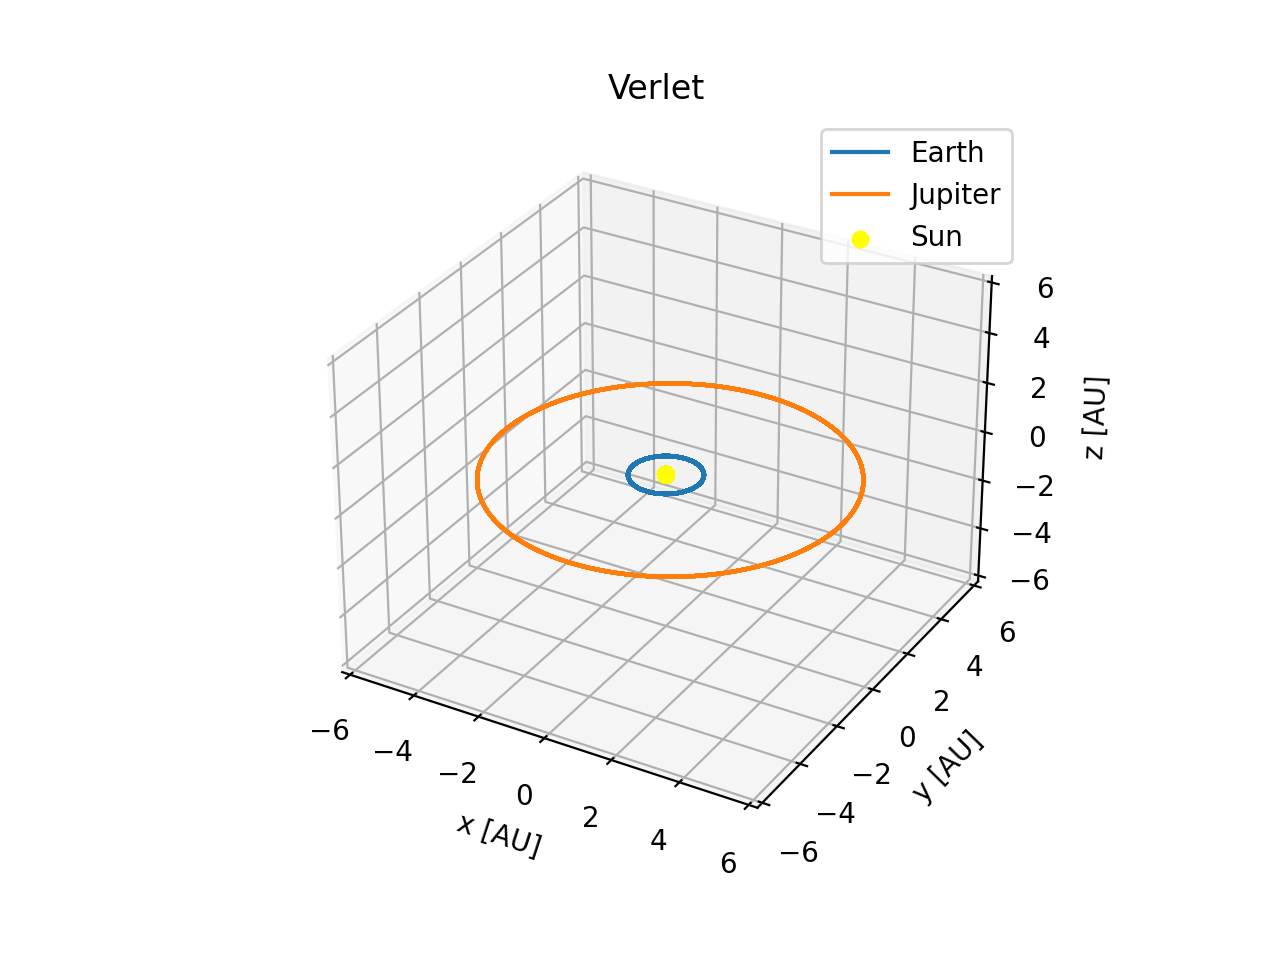
\includegraphics[width=1.15\linewidth]{Figure/threebodynormalmass120.png}
		\end{subfigure}
		\caption{3D plot of Jupiter's annual (left) and centennial (right) orbit around the Sun as calculated by the Velocity Verlet algorithm for respective temporal resolutions $h = 1.2\cdot10^{-5}$ and $h = 1.2\cdot10^{-4}$.}
		\label{jupiter12and120}
	\end{figure}
	\begin{figure}[h!]
		\centering
		\begin{subfigure}{0.45\linewidth}
			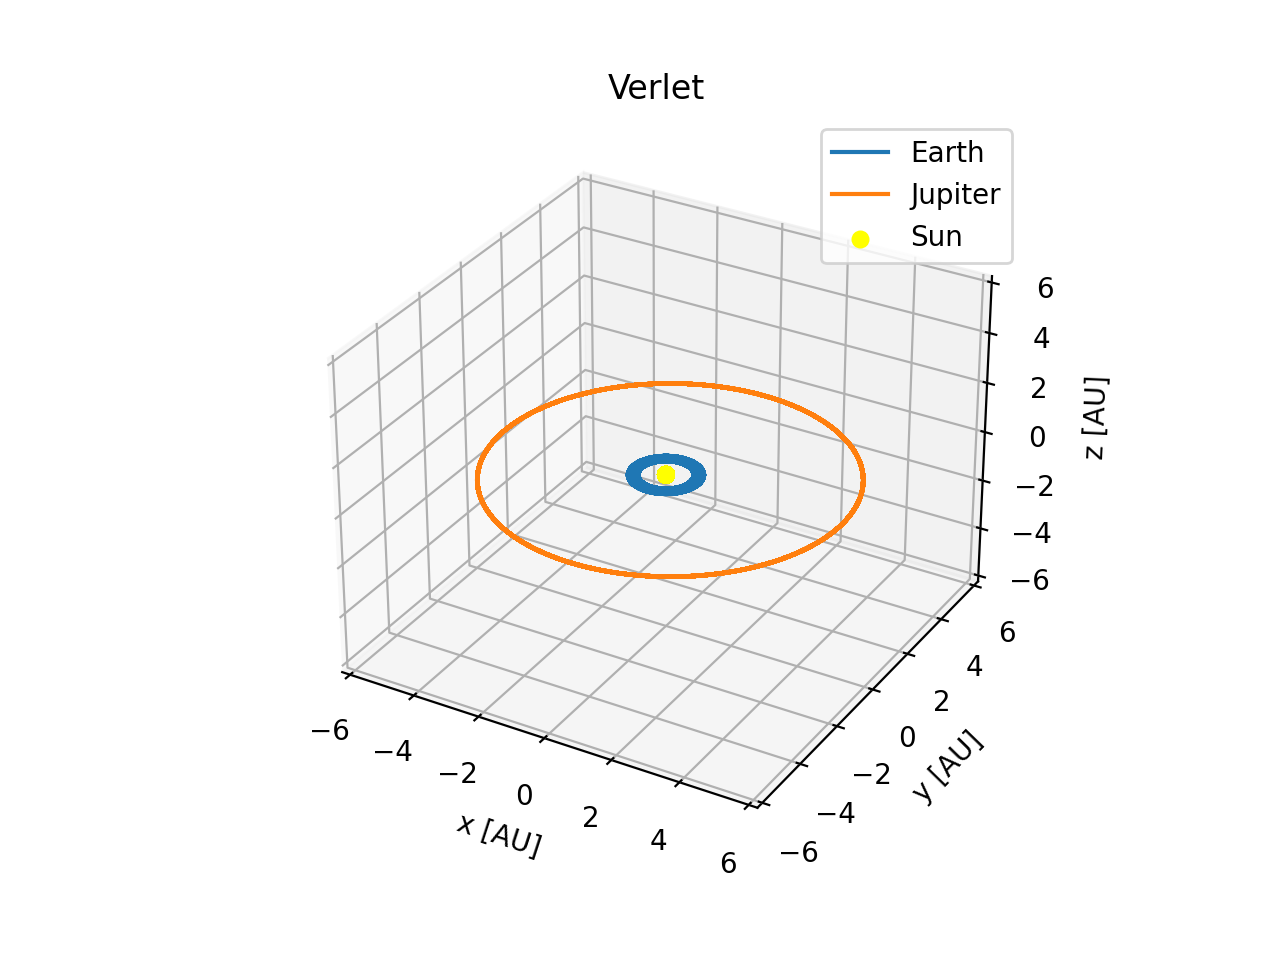
\includegraphics[width=1.2\linewidth]{Figure/threebodynormalmass1200.png}
		\end{subfigure}
		\begin{subfigure}{0.45\linewidth}
			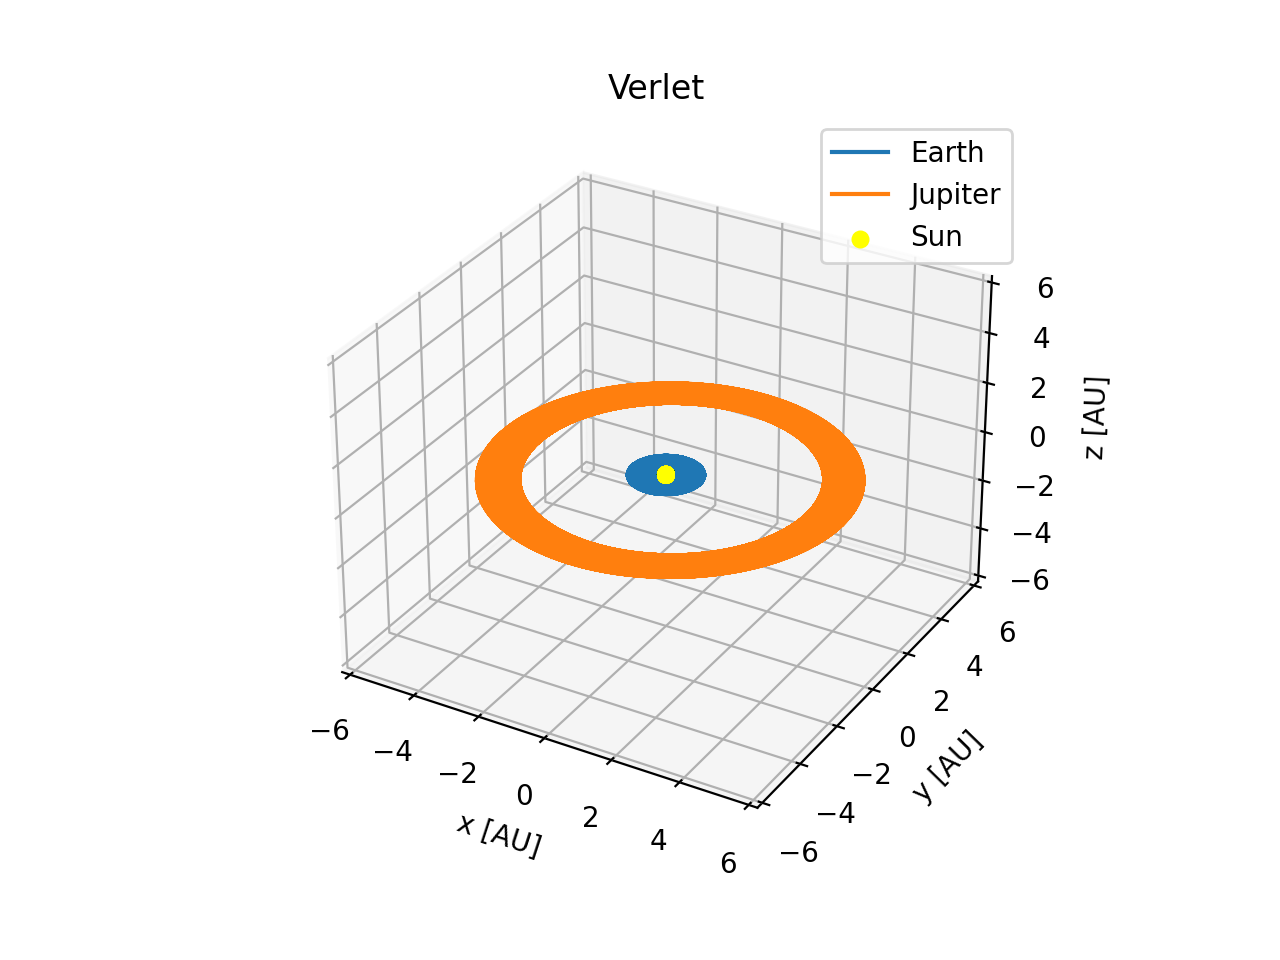
\includegraphics[width=1.2\linewidth]{Figure/threebodynormalmass12000.png}
		\end{subfigure}
		\caption{3D plots of Jupiter's millennial (left) and 12th millennial (right) orbit around the Sun as calculated by the Velocity Verlet algorithm for respective temporal resolutions $h = 1.2\cdot10^{-3}$ and $h = 1.2\cdot10^{-2}$.}
		\label{jupiter1200and12000}
	\end{figure}
	\newpage
	 Figures \ref{jupiter12and120} and \ref{jupiter1200and12000} are results obtained from simulating the motion of both the Earth and Jupiter for a system in which the Sun is fixed to the origin, devising the Velocity Verlet algorithm each time. Here we may observe that, much like for the binary Earth-Sun system, the semi-like\footnote{As the Sun is rigidly fixed, this is not a real three-body simulation, but the system exists however of three bodies.} three - body systems are well behaved for high temporal resolutions ($h < 10^{-3}$), and exhibit noticeable numerical imprecision for low temporal resolutions ($h > 10^{-3}$) as the orbital circumferences increase over time. Although this system is not a 'real' three-body system, it remains physically interesting as we may use it to study how Jupiter influences the motion of the Earth while still under the influence of the gravitational force it experiences from the Sun.
	 
    \begin{figure}[h!]
		\centering
		\begin{subfigure}{0.48\linewidth}
			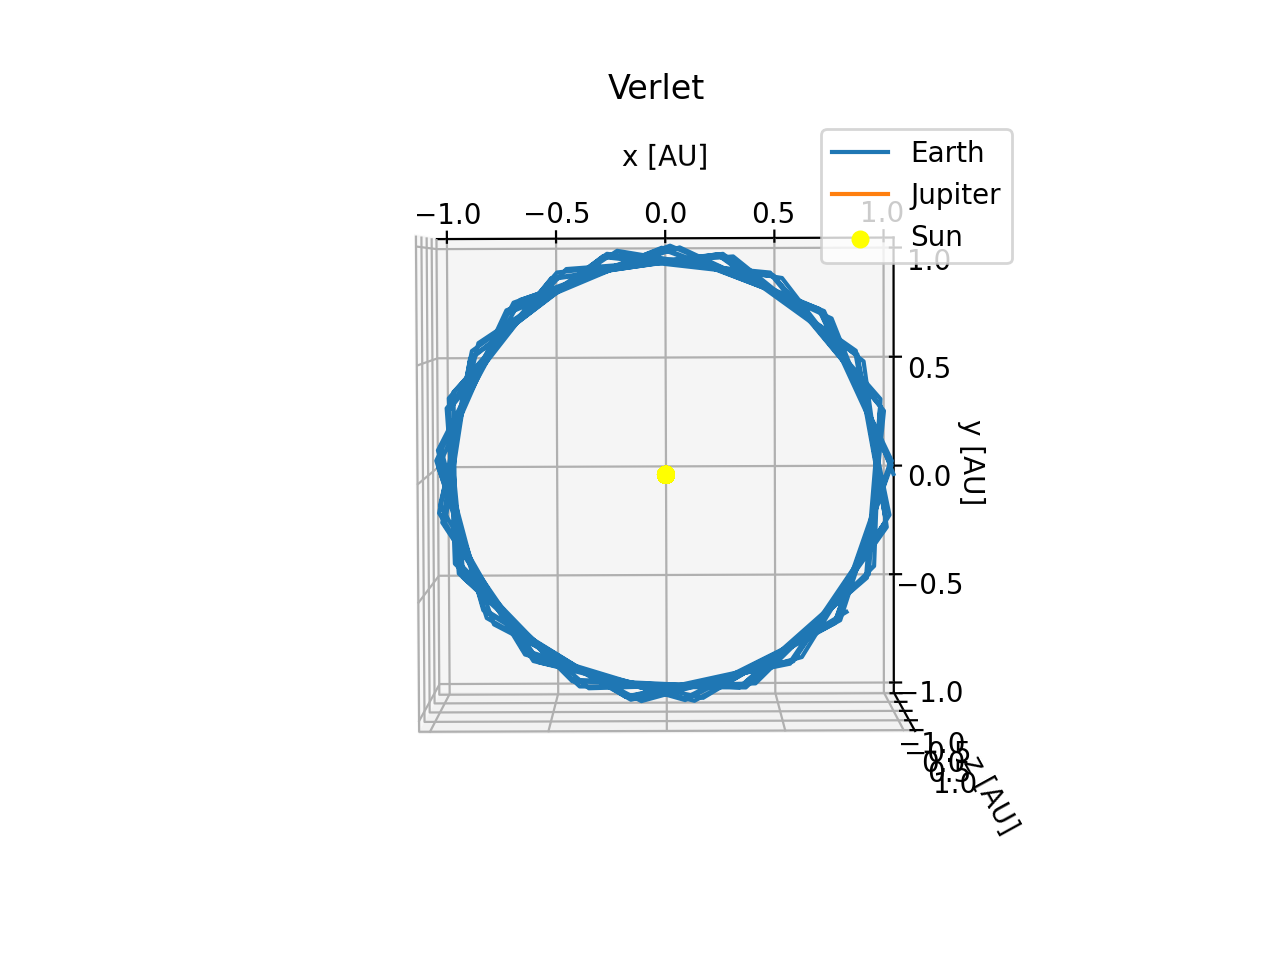
\includegraphics[width=1.2\linewidth]{Figure/threebody10mass12.png}
			\caption{12 years}
		\end{subfigure}
		\begin{subfigure}{0.48\linewidth}
			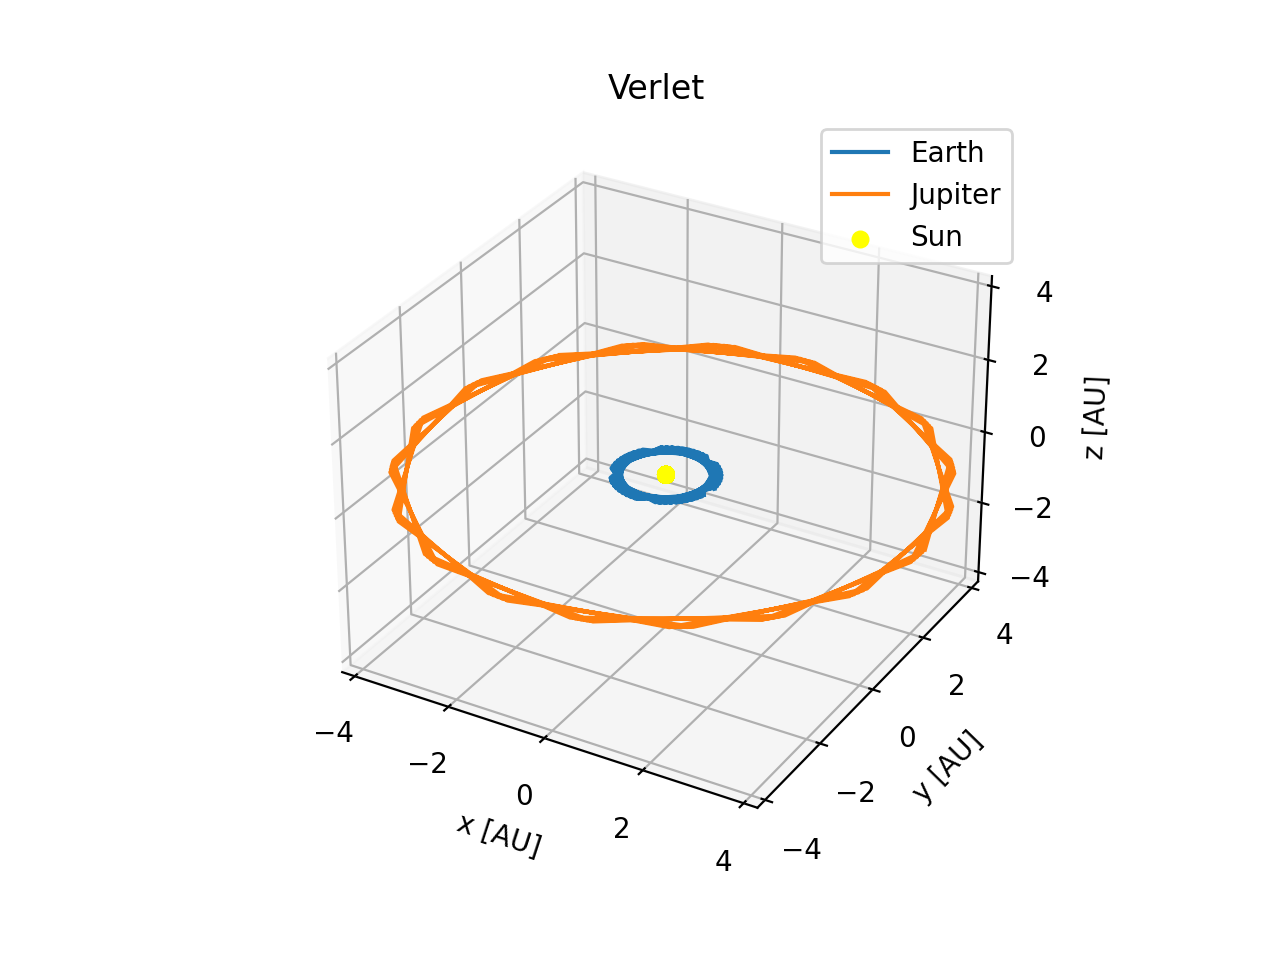
\includegraphics[width=1.15\linewidth]{Figure/threebody10120.png}
			\caption{120 years}
		\end{subfigure}
		\caption{3D plot of Earth's orbit while under influence of Jupiter (left) and Jupiter's orbit (right) with $h = 1.2\cdot10^{-5}$ and Jupiter's mass increased by a factor of 10}
		\label{jupitermass10}
	\end{figure}
	
	Figure \ref{jupitermass10} shows the system when Jupiter's mass is increased 10-fold. As can clearly be seen from the plots, this has a huge influence on Earth's orbit after 12 years, and an influence on Jupiter's orbit after 120 years.
	
	\begin{figure}[H]
    	\centering
    	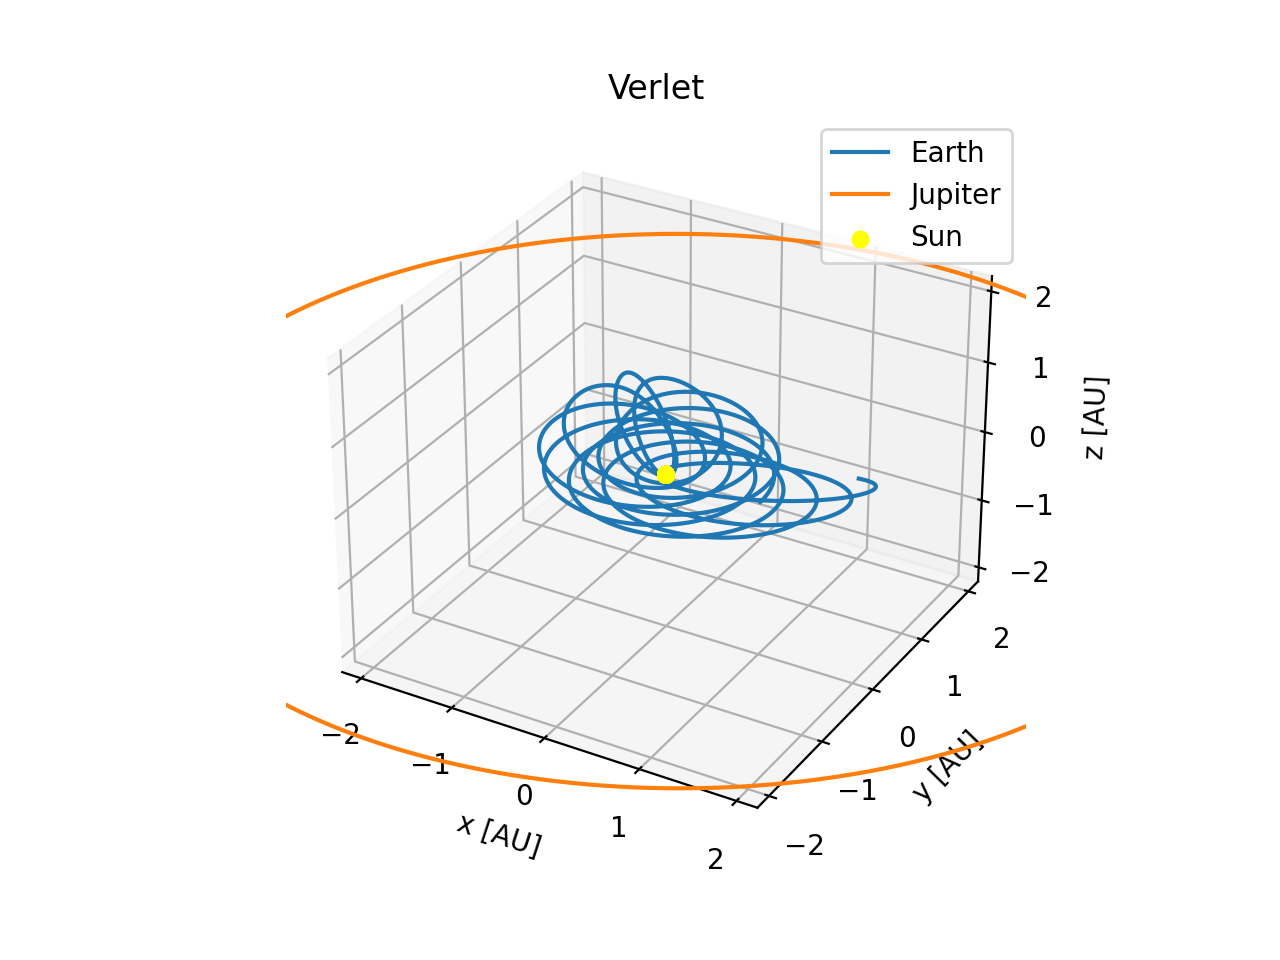
\includegraphics[width=\textwidth]{Figure/threebody1000mass12.png}
    	\caption{3D plot of the three-body system with Jupiter's mass increased by a factor of 1000}
    	\label{jupitermass1000}
	\end{figure}
	
	From Figure \ref{jupitermass1000}, Earth's orbit quickly deteriorates, and we've elected to leave out results for runs with larger final times, as 12 years is sufficient to illustrate that the system is no longer stable. 
	
	\subsection{The N-body System}
	Now we expand our model to contain all of the planets in the solar system and get the following result when we plot the position using the Velocity Verlet method:
	
	\begin{figure}[H]
    	\centering
    	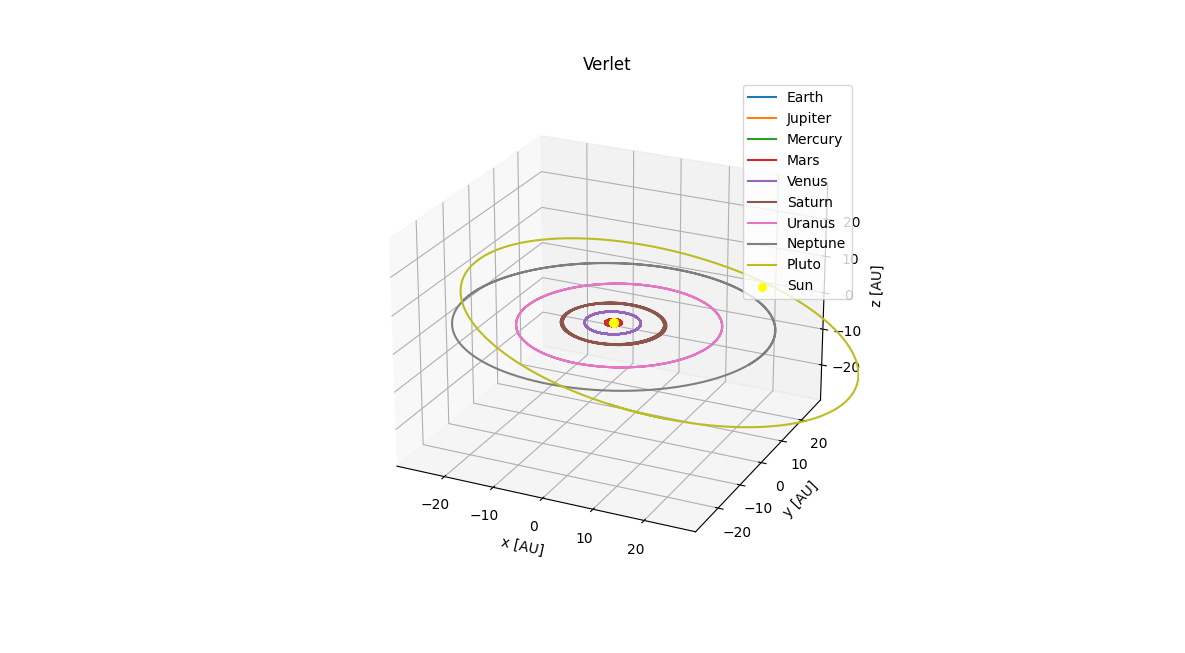
\includegraphics[width=\textwidth]{Figure/multibodyfixed250.png}
    	\caption{3D of the entire Solar system, including Pluto. No moons have been included. Time-span of 250 years, with $h=2.5\cdot10^{-4}$ and the Solar system Barycenter as origin.}
    	\label{nbody}
	\end{figure}
	
    Figure \ref{nbody} shows a spatial plot of all the planets in the Solar system, including Pluto, which is included for historical reasons. The system is plotted for a period of 250 years, which roughly corresponds to one revolution for Pluto. The origin is chosen as the centre-of-mass of the entire system, or the Solar system Barycenter. This has been done by using vector data from the JPL HORIZONS Web-Interface\cite{horizons}. This means that in this system, the Sun is unfixed and allowed to move.
    
    \subsection{Perihelion precession of Mercury}
    A function \texttt{VelocityVerletRel()} has been made which includes the correction term to the gravitational force described in \eqref{relativistic}. After the entire Velocity Verlet algorithm has been for one century, the function finds the position of Mercury at Perihelion in the 100th year, and prints these coordinates. We've run the program with the Sun both fixed to the origin, and unfixed, with the centre-of-mass as origin.
    
    \begin{table}[H]
		\centering
		\caption{Values of $\theta$, the angle of perihelion precession for Mercury after one century, Sun fixed to origin}
		\label{thetatableunfixed}
		\begin{tabular}{|l|l|l|}
		    \hline
			 & $\vartheta_P$ & Arc seconds\\
			\hline
			With relativistic correction term & $2.08\cdot10^{-3}$ & 429''\\
			Without relativistic correction term & $2.88\cdot10^{-3}$ & 594'' \\
			Absolute sum & $1.05\cdot10^{-4}$ & 165''\\
			\hline
	    \end{tabular}
	\end{table}
    
    \begin{table}[H]
		\centering
		\caption{Values of $\theta$, the angle of perihelion precession for Mercury after one century, centre-of-mass as origin}
		\label{thetatablefixed}
		\begin{tabular}{|l|l|l|}
		    \hline
			 & $\vartheta_P$ & Arc seconds\\
			\hline
			With relativistic correction term & $4.52\cdot10^{-4}$ & 93.2''\\
			Without relativistic correction term & $3.46\cdot10^{-4}$ & 71.2'' \\
			Absolute sum & $1.05\cdot10^{-4}$ & 22''\\
			\hline
		\end{tabular}
	\end{table}
	

	
The simulation was done with $h = 5\cdot10^{-5}$ for the results in Tables \ref{thetatablefixed} and \ref{thetatableunfixed}.
	
	
    
